\documentclass{article}

\usepackage{graphicx}
\usepackage{subfig}
\usepackage{float}
\usepackage{hyperref}
\usepackage{mathtools}
\usepackage[utf8]{inputenc}
\usepackage{biblatex}

\addbibresource{bibliography.bib}

\title{%
  Biometric Systems project \\
  \large DL based iris feature extractor trained with few-shot learning}
\author{Eduardo Rinaldi 1797800}
\date{}

\begin{document}

\maketitle

\tableofcontents
\newpage

\section{Introduction}
For my bachelor's thesis I decided to work on an iris recognition system which relies on $IS_{IS} \ v.2$ method for segmentation (Iris segmentation for Identification Systems) and both $LBP$ and $Spatiogram$ operators for feature extraction. For this project instead I decided to circle back and try other approaches regarding iris recognition (for both segmentation and feature extraction).


\subsection{Pipeline}

\begin{figure}[H]
    \centering
    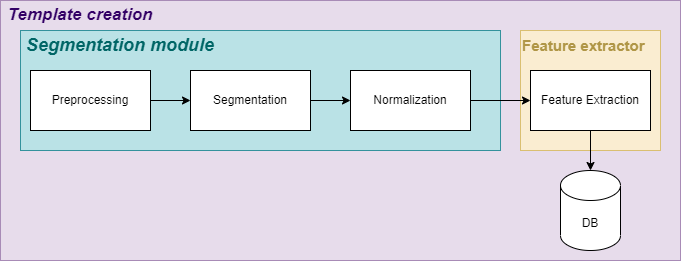
\includegraphics[width=5in]{imgs/MainPipeline.png}
    \caption{Main pipeline}
    \label{fig:MainPipeline}
\end{figure}

The pipeline is the \textit{``classical"} one, I just subdivided it in easy to change sub-modules:
\begin{itemize}
    \item \textbf{Segmentation}: 2 different segmentation modules, one which is $IS_{IS}\ v.2$ and another based on a slightly different approach that will be discussed later, for simplicity I'll name it in both this report and code as \textbf{ ``Hough approach"}. I decided to use only this latter for time limitation (obviously in the code I put both modules).
    \item \textbf{Feature Extraction}: 4 different feature extractors (only one is used in the demo, so no ensemble) all based on \textbf{deep learning approaches}; the main difficulty here lies in the training part because as will be explained in next section the dataset used is relatively ``small". Since I have decided to spend most of my time on this part and the approaches tested are quite ``recent" and ``unusual", the project is more focused on feature extraction.
\end{itemize}

\section{Technologies and libraries}
\begin{itemize}
    \item \textbf{Languages}: 
    \begin{itemize}
        \item \texttt{C++17} for segmentation, providing CMake file for compiling code as both executable and static library (in case someone want to use the segmentation module as an external library).
        \item \texttt{Python 3.9.4} for the whole pipeline and demo; I created a tiny API for calling the segmentation compiled executable from python.
        \item \texttt{IPython notebook} (hosted on \textit{Google Colab}), I provide python notebook that has been used for creating the feature extractor models. In this notebook all the steps are explained in details.
    \end{itemize}
    \item \textbf{Libraries}: OpenCV, PyTorch, Pandas, Numpy
\end{itemize}

In the section \textbf{``How to test the pipeline"} are explained all the steps needed to run each module and the demo.

\section{Dataset}
Due to limited time I decided to train and test the whole project on only one dataset which is
\href{https://utiris.wordpress.com/}{\textbf{Utiris}} \cite{HosseiniAraabiSoltanianZadeh:2010}. The database is constructed with 1540 images from 79 individuals from both right and left eyes demonstrated in 158 classes in total. The individuals are numbered the same in NIR and VW sessions, but for the feature extraction I only used VW images.

\subsection{Train - test split}
I decided to split the dataset giving \textbf{75\% of the subjects for training set} and the remaining \textbf{25\% for testing set}. Notice here that I \textbf{split by subjects} not by probes, so the final models will be evaluated on subjects they never seen (overfit can be easily spotted); the reason behind this choice lies in the training approach, but it will be explained and discussed in the \textit{``Feature extractors"} section.

\section{Segmentation modules}
As said before, segmentation modules provided here are two, but the code has been structured in such a way that I can implement a new one and then use it with rest of the pipeline. Indeed, these segmentation modules can be seen as a function that takes an image cropped on an eye and returns \textbf{two circles}: one for the \textbf{limbus} and one for the \textbf{pupil}, so in each module we're ``describing" how to find these two circles.
They share a common part which consists in:
\begin{enumerate}
    \item \textbf{Preprocessing}: this part is needed for \textbf{speeding up computation time} and for \textbf{removing reflections}. First, I find ROI (Region of interest) of the eye using an Haar Cascade classifier obtaining a ``squared" image, then I scale the image to a fixed size (in my case 250x250).
    \item \textbf{Normalization}: given as input limbus and pupil circle to normalization module we obtain an image normalized following the rubber sheet model. (Example of normalized iris in fig \ref{fig:rsm})
\end{enumerate}

\begin{figure}[H]
    \centering
    \subfloat[Rubber sheet model]{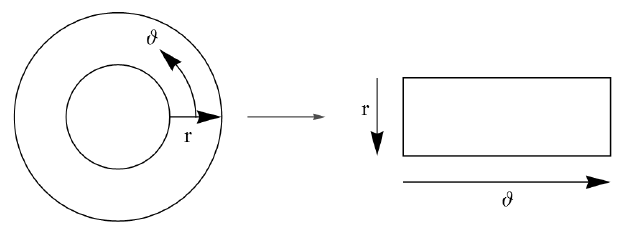
\includegraphics[width=2.5in]{imgs/daugman.png}}\\
    \subfloat[Normalized iris]{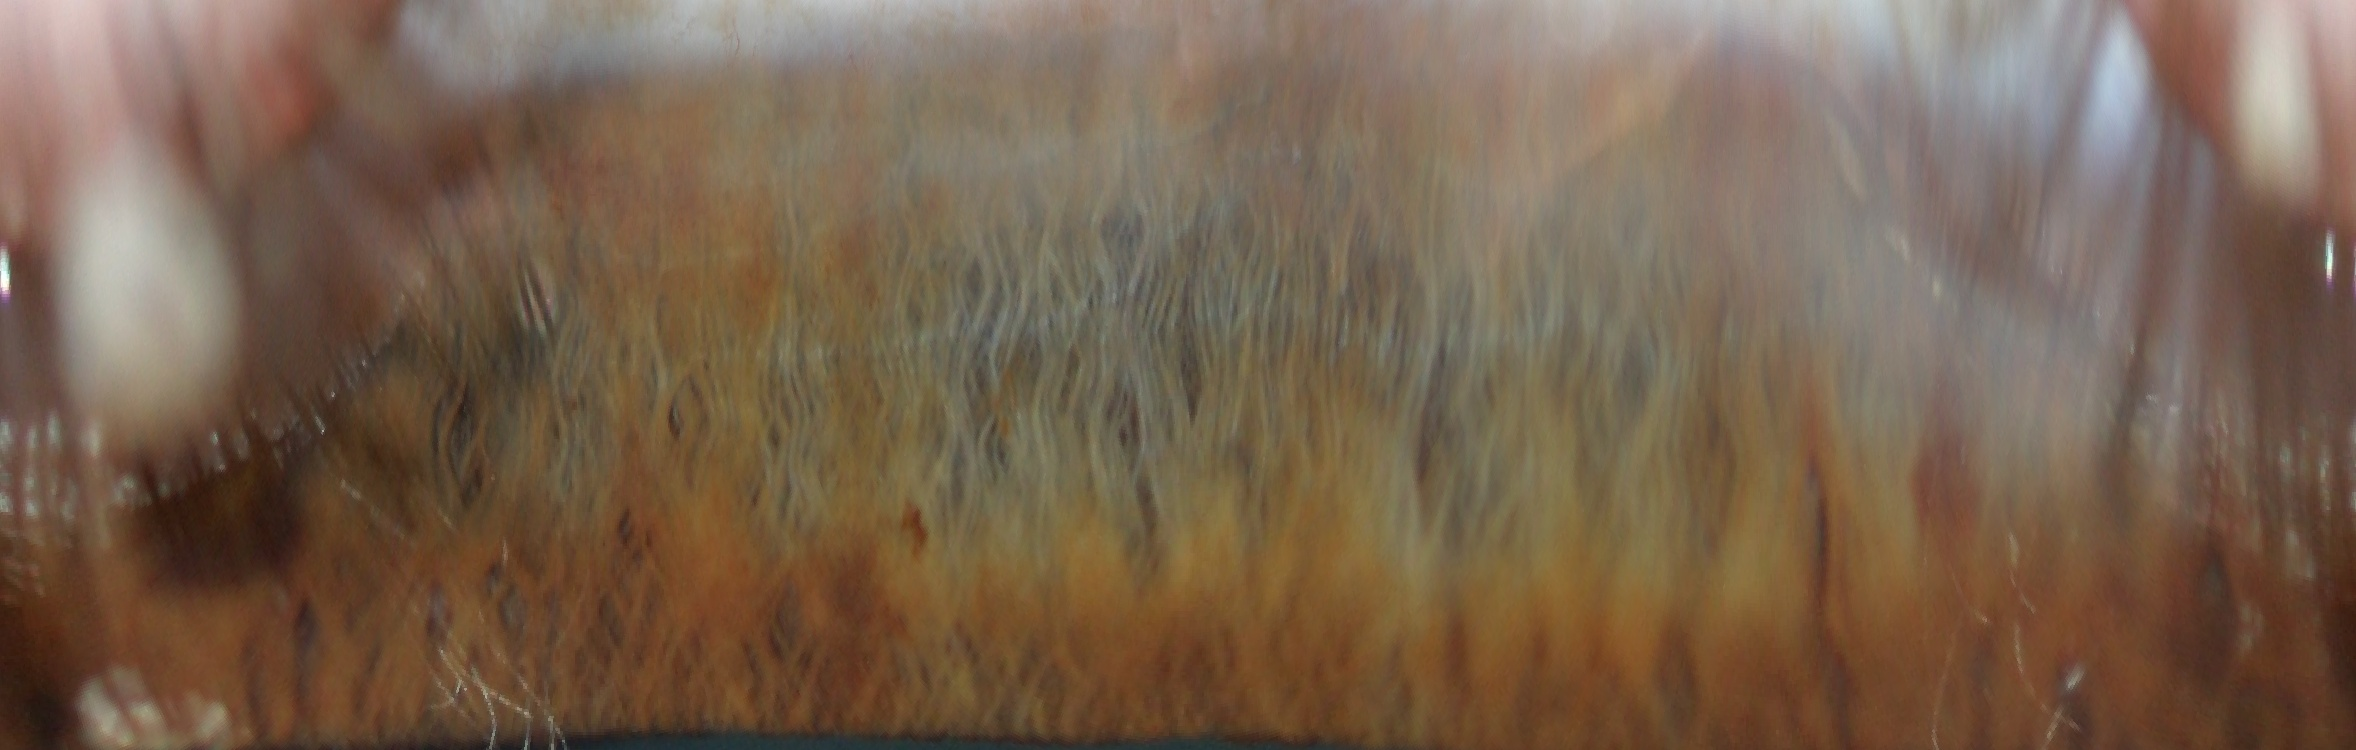
\includegraphics[width=2in]{imgs/normalizedImage.JPG}}
    \caption{Iris normalization}
    \label{fig:rsm}
\end{figure}

\subsection{$IS_{IS} v2$}
The main idea behind this module is to find \textbf{first the limbus} and \textbf{then the pupil} using a \textbf{``bruteforce" approach}. For bruteforce here I mean that every time the algorithm try to find one of the two circles it first generates all the possible ones using different parameters and then select the best circle according to a specific metric. So we can subdivide the ``circle finding" in two main big steps: \textit{``circle candidates generation"} and \textit{``circle selection"}.

\subsubsection{Circle candidates generation}
In this step, in order to increase the contrast in the image, a \textbf{posterization filter} is applied to the preprocessed image. The filter consists in:
\begin{enumerate}
    \item Convert image in gray scale
    \item A window $W$ of size $(2k + 1)\times (2k + 1)$ is scrolled over the entire image, and at each scrolling a histogram $H_W$ is calculated on the pixels inside $W$
    \item The most frequent colour within $H_W$ is assigned to the central pixel of $W$
\end{enumerate}

At every iteration, $k$ is increased (ranging in $[1, 17]$).

After this ``preprocessing" step a list of edges are detected using \textbf{``Canny edge detector"} and these are then given as input to a circle fitting algorithm (for this module is the \textbf{Taubin} method) which will output a list of candidates circles.

\subsubsection{Circle selection}
This step receives as input a list containing all the candidates circles obtained after each iteration of the previous step and returns only one circle based on some criteria:
\begin{itemize}
    \item For limbus circle we have the following constraints:
    \begin{itemize}
        \item $ size_{img}*0.15 \leq radius_{limbus} \leq size_{img}*0.5$
        \item must have the higher score (based on \textbf{homogeneity} and \textbf{separability})
    \end{itemize}
    \item For pupil circle we have the following constraints:
    \begin{itemize}
        \item $diameter_{limbus}*0.1 \leq radius_{pupil} \leq diameter_{limbus}*0.2$
        \item must be inside the limbus circle
        \item must have the higher score (based on \textbf{homogeneity} and \textbf{separability})
    \end{itemize}
\end{itemize}

\subsection{Hough approach}
This approach is a custom one created by mixing some of the approaches used in $IS_{IS}$ and some of the ones used \href{https://github.com/andreibercu/iris-recognition}{here} (this latter is thought to work well on infrared images).

\bigskip
The main idea here is to find \textbf{first the pupil} and \textbf{then the limbus} still using a ``bruteforce" approach based on \textit{``circle candidates generation"} and \textit{``circle selection"} steps.

\subsubsection{Circle candidates generation}
This step starts by transforming the input image in gray scale for then apply a \textbf{median blur filter} (at each iteration the size of the window used by the filter is increased), this helps reducing noise in the image.

\bigskip
Then as in $IS_{IS}$, I use \textbf{canny edge detector} for obtaining circle edges. 

When the algorithm is looking for pupil circles I apply the following ``trick": since pupil circle is composed by very dark pixels, I can inverse threshold the blurred image with small threshold values (at each iteration this threshold is increased) for then giving the resulted image to the canny edge detector; this latter in this case will have more chances to detect edges of pupil. 

\begin{figure}[H]
    \centering
    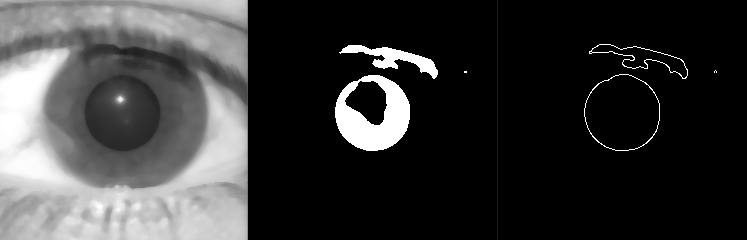
\includegraphics[width=4.5in]{imgs/threhsolded.PNG}
    \caption{From left to right: blurred image, thresholded image, edge detected by canny}
    \label{fig:thresholded}
\end{figure}

Instead when the algorithm is looking for limbus circle, the edge detector receives as input the blurred image.

\bigskip
Final step consists in giving the \textit{``edge map"} (i.e. the output of canny) as input to \textbf{``Hough circle transform"} which will give as output a list of all possible circles (something "similar" to \textbf{Taubin} circle fitting).
At each iteration we decrease the \textit{``param2"} parameter of Hough transform, which is the accumulator threshold, the smaller it is the more false circles may be detected (it ranges in $[35, 120]$).

\subsubsection{Circle selection}
This step for \textbf{pupil} is very simple: just take the mean circle (i.e. mean position and mean radius).

For \textbf{limbus} a filtering process is applied: 
\begin{enumerate}
    \item every circle with $radius_{limbus} < 1.5*radius_{pupil}$ is discarded from the ``candidates" list.
    \item every circle positioned outside pupil circle is discarded from the ``candidates" list. 
    \item mean circle $\mu$ and std circle $\sigma$ are calculated, then every circle with position or radius outside the range $[\mu - 1.5 \sigma, \mu + 1.5 \sigma]$ is discarded from the ``candidates" list. 
\end{enumerate}

At the end of this filtering process, as for pupil, the \textit{new} mean circle among the candidates is taken.

\section{Feature extractors}
Since the project focuses more on feature extraction and since the methods proposed are fairly recent and therefore seem to be underused, this section will be the one with the most detail.

\bigskip
All code concerning this section and the evaluation phase can be found in the python notebook \texttt{"Iris Feature Extraction.ipynb"}, together with the code various explanations of each step are given.

\subsection{Preface} 
Initially, the idea was to use pretrained networks such as \textit{vgg}, \textit{densenet} and \textit{resnet} and then perform a fine-tuning operation for the proposed dataset. This idea was immediately catalogued as a failure for two main reasons:
\begin{itemize}
    \item for each class there are very \textbf{few examples} (about 5), not enough even for a small fine-tuning process
    \item if a new subject is added to gallery we need to retrain the whole model (this occurs only if these models are used as ``end" classifiers)
\end{itemize}

This was the starting point for my research into possible ``training techniques" that could fit well with my needs: it was here that I came across two ``techniques" called \textbf{\textit{``few-shot learning"}} and \textbf{\textit{``siamese networks"}}.

\subsubsection{Few-shot learning}
Few-shot learning is the problem of making predictions based on a limited number of samples.
The goal here is not to let the model recognize the images in the training set and then generalize to the test set, instead, the goal is to learn (\textit{“learn to learn”}).

\bigskip
Let's do an example: let's suppose that we have as training set the images in figure \ref{fig:exampleTS}

\begin{figure}[H]
    \centering
    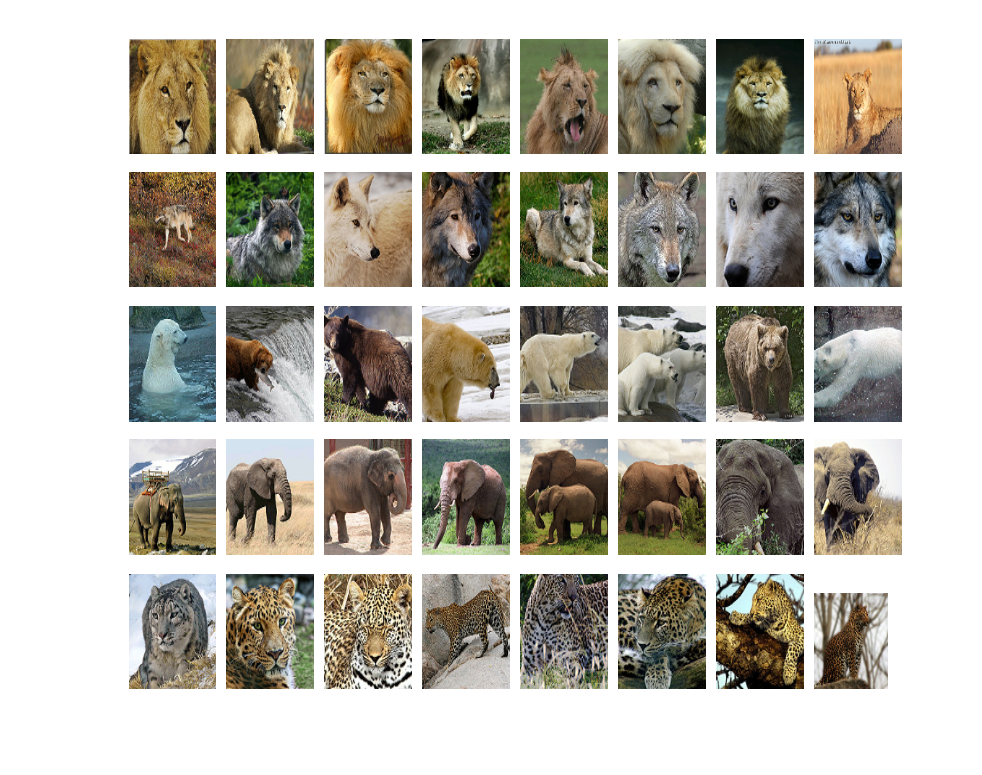
\includegraphics[width=4in]{imgs/Wild_Anima_dataset.png}
    \caption{Example training set}
    \label{fig:exampleTS}
\end{figure}

The goal of training is not to know what an elephant is and what a tiger is but instead, the goal is to \textbf{know the similarity and difference between objects}. So, later, I can give two images of animals that never appeared in the training set and the model can say if they are the same animal (it learns a similarity/distance measure).

\begin{figure}[H]
    \centering
    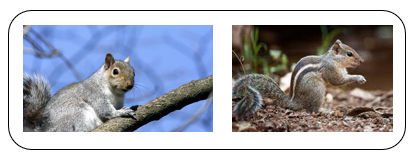
\includegraphics[width=4in]{imgs/squirrel.png}
    \caption{Test pair}
    \label{fig:exampleTP}
\end{figure}
Let's now go back to our example; when the model sees the pair of images in figure \ref{fig:exampleTP} it does not know they are squirrels (we didn't train the model to recognize the class). However, the model can tell you with high confidence that they are the same kind of objects. This technique seems to be \textbf{well suited for biometric recognition models}.

\subsubsection{Siamese Networks}
A possible implementation of few-shot learning is through to the concept of Siamese networks \cite{koch2015siamese}, which consists of twin networks (generally two or three) which accept distinct inputs but are joined by an energy function and they share the same weights, this guarantees that two extremely similar images are not mapped by each network to very different locations in feature space because each network computes the same function. After the training phase we can then extract the network used at the base, i.e. the one that produces the feature vector, and use it as a ``feature extractor" (I will use this term in the next sections to refer to the network at the base).

\bigskip
For this project I decided to try two different architectures of siamese networks: \textbf{pair siamese networks} and \textbf{triplet siamese network}, both based on conv. neural networks.

\paragraph{Pair siamese networks}

During training, as the name suggests, an image pair is fed into the model with their ground truth relationship $y$: $y = 1$ if the two images are similar and 0 otherwise. The loss function for a single pair is the \textit{contrastive loss}:

$$yd^2 + (1 - y) max(m - d, 0)^2$$

where:
\begin{itemize}
    \item $d$ is the euclidean distance between the two feature vectors obtained by the network
    \item $m$ is called margin, is used to “tighten” the constraint: if two images in a pair are dissimilar, then their distance should be at least $m$, or a loss will be incurred
\end{itemize}

\begin{figure}[H]
    \centering
    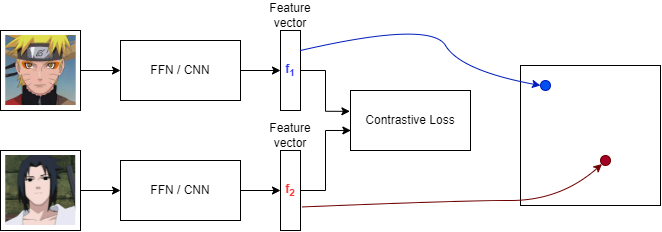
\includegraphics[width=4.5in]{imgs/pairNet.png}
    \caption{Example of pair siamese network}
    \label{fig:pairNet}
\end{figure}

\paragraph{Triplet siamese networks}
During training process, an image triplet $<I_a, I_p, I_n>$ is fed into the model as a single sample, where $I_a$, $I_p$ and $I_n$ represent the anchor, postive and negative images respectively. The idea behind is that distance between anchor and positive images should be smaller than that between anchor and negative images.
The loss function used is called \textit{triplet loss}:

$$max(\left\| f_a - f_p\right\|^2 - \left\| f_a - f_n\right\|^2 + m, 0) $$

\begin{figure}[H]
    \centering
    \includegraphics[width=4.5in]{imgs/TripletNet.png}
    \caption{Example of triplet siamese network}
    \label{fig:tripletNet}
\end{figure}

\begin{figure}[H]
    \centering
    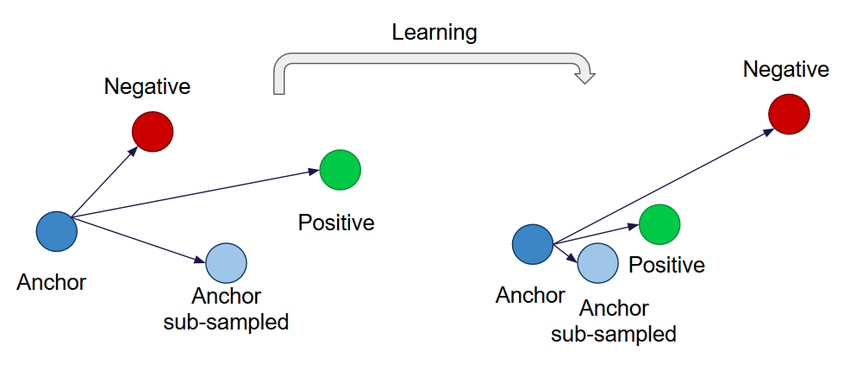
\includegraphics[width=4in]{imgs/Scheme-of-the-learning-process-of-our-adapted-triplet-loss-function-See-the-Equation-6.png}
    \caption{Triplet loss}
    \label{fig:tripletNet}
\end{figure}

\subsection{Trained and tested models}
Now that I have explained, although in a very simple way, the underlying mechanism, I can list the feature extractors trained and tested:
\begin{enumerate}
    \item \texttt{vggFEPair}: pretrained model of vgg fine-tuned using pair few-shot learning (pair siamese network)
    \item \texttt{vggFETriplet}: pretrained model of vgg fine-tuned using triplet few-shot learning (triplet siamese network)
    \item \texttt{vggFEPretrained}: pretrained model of vgg as it is, no fine-tuning applied, used as feature extractor
    \item \texttt{featNetTriplet}: inspired by \textit{featNet} architecture in \cite{9036930}, but most important \textbf{trained from scratch} (weights are initialized randomly)
\end{enumerate}

Training was done for 100 epochs.

\section{Evaluation}
For the evaluation phase I measured the performance of the different models on:
\begin{itemize}
    \item \textbf{All-vs-all verification} multiple template, obtaining 3 main informations: \textit{FAR}, \textit{FRR} and \textit{EER}.
    \item \textbf{All-vs-all identification} open-set multiple template, obtaining the following main informations: \textit{FAR}, \textit{FRR}, \textit{EER}, \textit{DIR} (Detection and Identication Rate) and \textit{CMS} (Cumulative Match Score)
\end{itemize}

To simplify the test phase, I calculated the distance matrix between all samples in the test set, using the Euclidean distance (distance values are not normalized). In the following sections the results obtained for each model will be presented.

\subsection{\texttt{vggFEPretrained}}
\begin{figure}[H]
    \centering
    \subfloat[Verification]{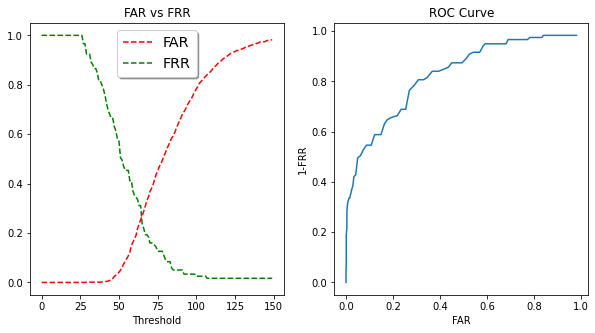
\includegraphics[width=4in]{imgs/vggFEPretrainedVerification.png}}\\
    \subfloat[Identification]{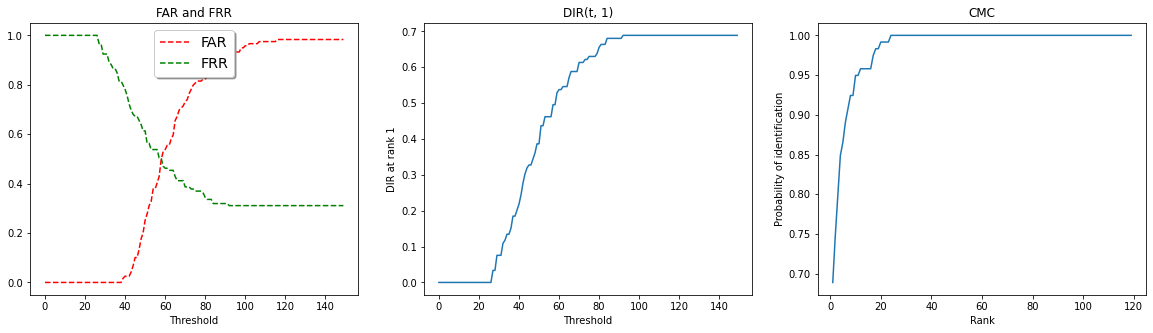
\includegraphics[width=5.5in]{imgs/vggFEPretrainedIdentification.png}}
    \caption{pretrained model of vgg as it is, no fine-tuning applied, used as feature extractor}
    \label{fig:vggFEPretrainedRes}
\end{figure}

\subsection{\texttt{vggFEPair}}

\begin{figure}[H]
    \centering
    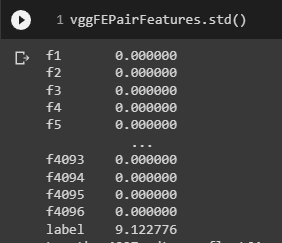
\includegraphics[width=2.5in]{imgs/vggFEPairStd.PNG}
    \caption{Standard deviation of feature extracted}
    \label{fig:vggFEPairStd}
\end{figure}

As can be seen in figure \ref{fig:vggFEPairStd}, the standard deviation on each feature is rounded to 0; this suggests that the features extracted from this model may not be so distant from each other. We can see this as a first red flag.

\begin{figure}[H]
    \centering
    \subfloat[Verification]{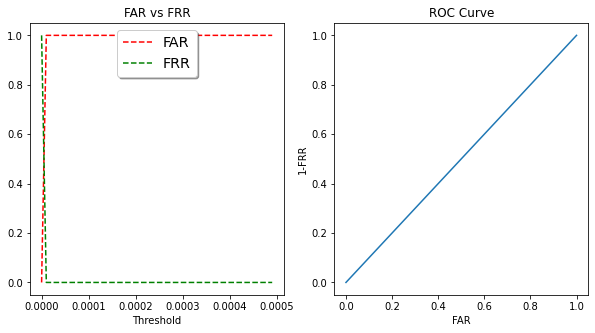
\includegraphics[width=4in]{imgs/vggFEPairVerification.png}}\\
    \subfloat[Identification]{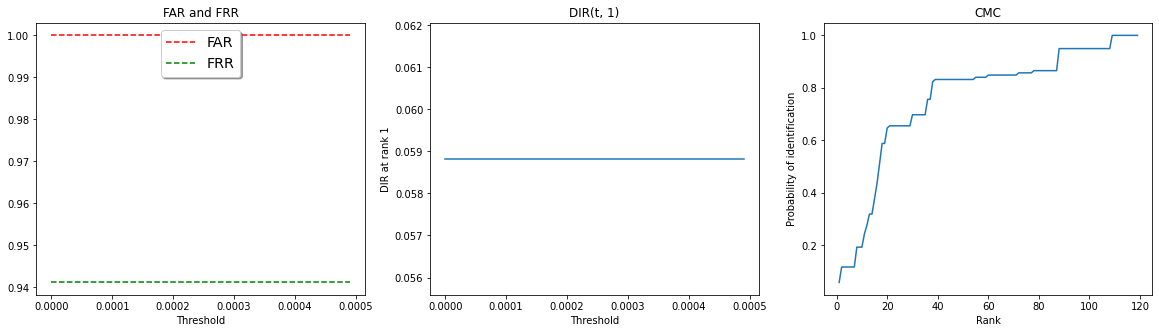
\includegraphics[width=5.5in]{imgs/vggFEPairIdentification.png}}
    \caption{pretrained model of vgg fine-tuned using pair few-shot learning (pair siamese network)}
    \label{fig:vggFEPairRes}
\end{figure}

\subsection{\texttt{vggFETriplet}}

\begin{figure}[H]
    \centering
    \subfloat[Verification]{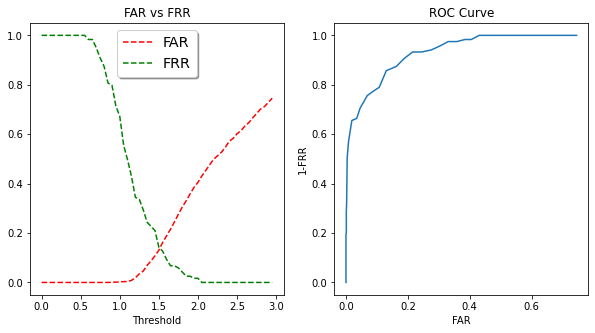
\includegraphics[width=4in]{imgs/vggFETripletVerification.png}}\\
    \subfloat[Identification]{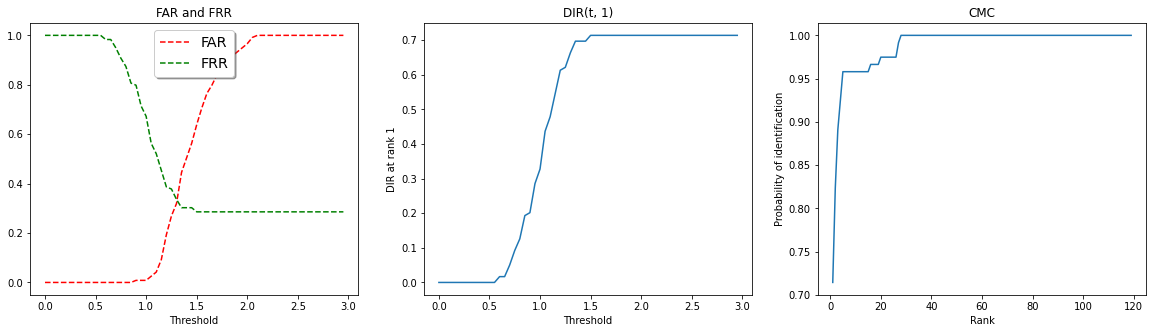
\includegraphics[width=5.5in]{imgs/vggFETripletIdentification.png}}
    \caption{pretrained model of vgg fine-tuned using triplet few-shot learning (triplet siamese network)}
    \label{fig:vggFETripletRes}
\end{figure}


\subsection{\texttt{featNetTriplet}}

\begin{figure}[H]
    \centering
    \subfloat[Verification]{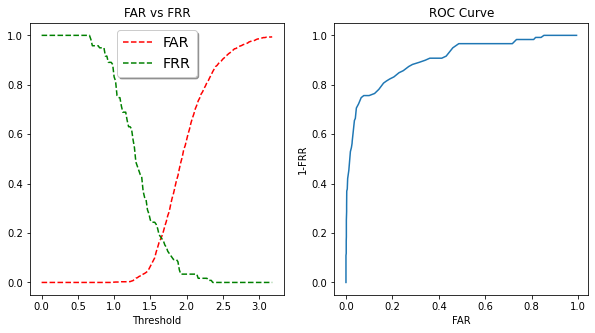
\includegraphics[width=4in]{imgs/featNetTripletVerification.png}}\\
    \subfloat[Identification]{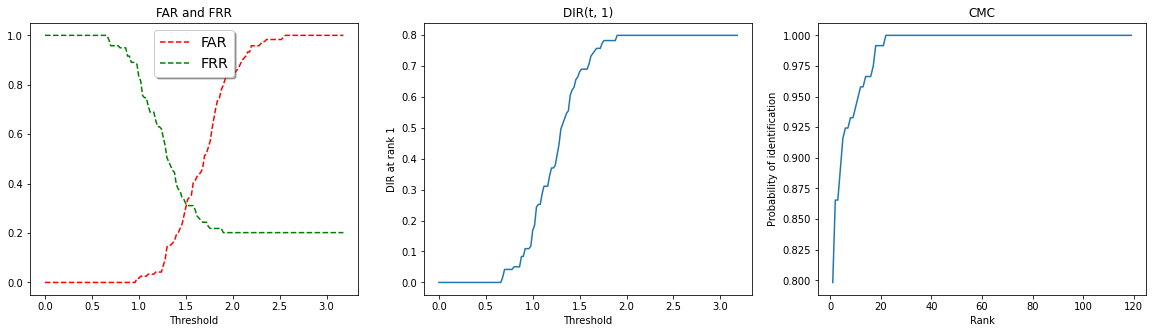
\includegraphics[width=5.5in]{imgs/featNetTripletIdentification.png}}
    \caption{inspired by \textit{featNet} architecture}
    \label{fig:vggFETripletRes}
\end{figure}

\subsection{Considerations after evaluation}
After this evaluation phase we can take several considerations:
\begin{itemize}
    \item \texttt{vggFEPretrained} (i.e. vgg without any kind of training/fine-tuning), compared to others, does not perform so bad on verification ($EER = {\sim} 0.25$).
    \item The best model for a verification task is \texttt{vggFETriplet}, since the $EER={\sim}0.16$. Note that a valid second choice could be \texttt{featNetTriplet} with $EER={\sim}0.2$, this result is amazing since the network has been trained from scratch.
    \item The best model for an identification task is \texttt{featNetTriplet}, with 
    \begin{itemize}
        \item $EER={\sim}0.3$ at $t=1.5$
        \item $DIR(t=1.5, 1)={\sim}0.7$ 
        \item $CMS(rank=1)=0.8$
    \end{itemize}
    \item Triplet training performs way better than pair training. This is probably due to the fact that in the first one the training phase on a single step tries to minimize distance between similar objects while maximizing the distance between different objects.
\end{itemize}

\section{Demo}
The demo consists of 3 python scripts on CLI:
\begin{itemize}
    \item \texttt{"Enrollment.py"} to perform enrollment of a subject in a specific ``db" (actually it is a simple csv file) specifying the input image and the associated identity
    \item \texttt{"Verification.py"} to perform a verification operation by specifying the input image and the claimed identity. At the end of this operation it will print the outcome: \textit{``Identity verified, you are user\#ID"} or \textit{``Access denied"}.
    \item \texttt{"Identification.py"} to perform an identification operation by specifying the input image. At the end of this operation it will print the outcome: \textit{``You are user\#ID"} or \textit{``No match in dataset"}.
\end{itemize}

For simplicity in the demo I decided to use only one model, specifically \texttt{featNetTriplet} (this can easily be changed with another), because is the most versatile and above all the file containing the pytorch model is only a few kilobytes. 

\bigskip
Instructions for using this demo are in \texttt{"README.md"} file.

\section{Future work}
Since time was limited and I didn't have any colleagues to work with, I had to choose what to do and what to not do; here I list several things that could be interesting to test:
\begin{itemize}
    \item Train and test all 4 feature extractors on a mixed dataset (e.g. \textit{Ubiris} + \textit{Utiris} + \textit{MICHE})
    \item Plug different feature extractors: could be a different pretrained network (e.g. densenet), or a custom network to train from scratch
\end{itemize}
\printbibliography
\end{document}
